\documentclass[12pt,oneside,openany,letterpaper]{article}


\usepackage{fancyhdr}
\usepackage{helvet}
\usepackage{amsmath}
%\usepackage{graphicx}
\usepackage[pdftex]{graphicx}
\usepackage{psfrag}
\usepackage{setspace}
%\usepackage[hypertex, linktocpage]{hyperref}[2003/11/30]
\usepackage[linktocpage]{hyperref}[2003/11/30]
\usepackage{lscape}
\usepackage{nicefrac}
\usepackage{mathrsfs}
\usepackage{units}
\usepackage{upgreek}
\usepackage{amssymb}
\usepackage{color}
\usepackage{wrapfig}
\usepackage{multirow}
\usepackage{url}
\usepackage{verbatim}
\usepackage{textcomp}
\usepackage{epstopdf}

\onehalfspacing \setlength\textheight{667pt}
\setlength\textwidth{506pt} \setlength\oddsidemargin{-18pt}
\setlength\topmargin{-20pt}
%\setlength\footskip{24pt}
\addtolength\headheight{2.5pt} \addtolength\headsep{-14pt}
%\fancyhead[R]{\includegraphics[height=10.5pt]{ubclogo_bw.eps}\#:  55907968}
%\renewcommand\familydefault{\sfdefault}
\pagestyle{empty}

\newenvironment{packed_enum}{
\begin{enumerate}
  \setlength{\itemsep}{0pt}
  \setlength{\parskip}{0pt}
  \setlength{\parsep}{0pt}
}{\end{enumerate}}



\fancyhead[L]{\emph{Introduction to Electronics}}\fancyhead[R]{$LRC$ Transients and Resonance}
\fancyfoot[L]{PHYS 231}\fancyfoot[R]{Experiment 2}
\pagestyle{fancy} \pagenumbering{arabic}

\begin{document}
\thispagestyle{plain}
\begin{center}
{\large{\bf{\fontfamily{phv}\selectfont Physics 231 - Ohm's Law \& the Kirchhoff Loop and Junction Laws  (Exp.~2)}}}
\end{center}

\noindent The purpose of this experiment is to test a few of the basic laws governing electric circuits, at the same time giving you more practice at setting up circuits and operating the instruments.

~


{\bf Part 2 - Ohm's Law}

~

\noindent Ohm’s law states that the current in a resistor is proportional to the voltage applied across it, $V = IR$, where the constant relating the two is the resistance $R$, measured in ohms ($1\rm\ \Omega = 1\rm\ V/A$). Pick a resistor with $50~\Omega\le R\le 100\rm\ k\Omega$ and assemble the following circuit:
\begin{figure}[h!]
\begin{center}
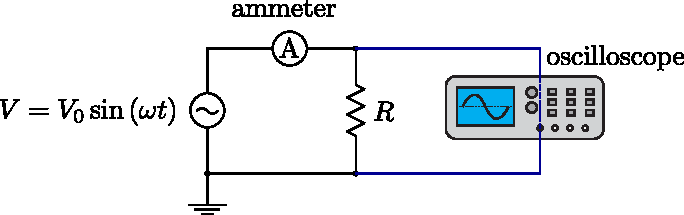
\includegraphics[width=.7\textwidth]{figures/Lab2Fig1.pdf}\caption{\label{fig:fig1}The circuit used to test Ohm's law.  The ammeter used to measure current must be placed in series with $R$ and the function generator.  The oscilloscope is used to measure the voltage across $R$ and must be placed in parallel with $R$.  The figure of the oscilloscope was taken from \href{https://commons.wikimedia.org/wiki/File:Symbol_oscilloscope.svg}{Wikimedia Commons}.}
\end{center}
\end{figure}

~

\noindent Set the digital multimeter (DMM) to measure AC current and use the oscilloscope to determine the voltage across the resistor. Test Ohm’s law using not just at one value of the function generator amplitude, but at several voltages to show that the $I$–$V$ relationship is linear. Do a weighted linear least squares fit to your data using the Jupyter notebook linked in the course website.


\clearpage


{\bf Part 2 - Kirchhoff's Voltage Loop Law}

~

\noindent Assemble the circuit below using three resistors of your choice. Use the DMM to test Kirchhoff’s voltage loop law around the loops in the circuit.  Select resistors with values between $50~\Omega\le R\le 100\rm\ k\Omega$.  

\begin{figure}[h!]
\begin{center}
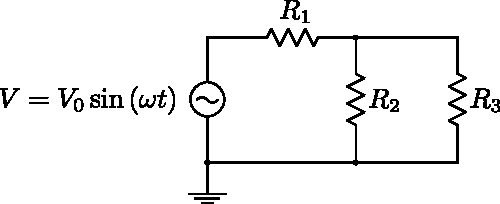
\includegraphics[width=.5\textwidth]{figures/Lab2Fig2.pdf}\caption{\label{fig:fig2}The circuit used to test Kirchhoff's voltage loop law.}
\end{center}
\end{figure}


~


{\bf Part 3 - Kirchhoff's Current Junction Law}

~

\noindent Assemble a circuit with a parallel combination of a $100\rm\ \Omega$ resistor and a $1000\rm\ \Omega$ resistor.  Connect the combination to the function generator and then insert the DMM into the circuit in various places in order to test Kirchhoff’s current junction law at the nodes in the circuit.

~

{\bf Part 4 - Kirchhoff's Voltage Law and Phase}

~

\noindent Assemble the series combination of a resistor and a capacitor shown below and set the function generator frequency to $f = \omega/\left(2\pi\right) = 16\rm\ kHz$. Use your DMM to once again check Kirchhoff’s voltage law around the loop. If you see a serious discrepancy, check the actual AC signals on the oscilloscope. In particular, look at the voltage across the capacitor and the voltage supplied by the generator simultaneously to compare the phases of the voltages.

\begin{figure}[h!]
\begin{center}
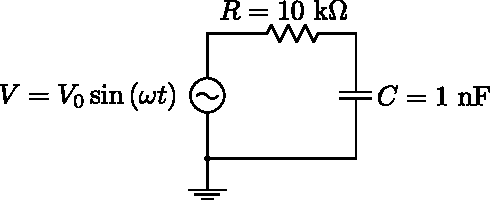
\includegraphics[width=.5\textwidth]{figures/Lab2Fig3.pdf}\caption{\label{fig:fig3}The circuit used to test Kirchhoff's voltage loop law in an $RC$ circuit.}
\end{center}
\end{figure}

\end{document}
